\documentclass[a4paper,12pt]{article}
\usepackage{tkz-euclide}
\usepackage{gensymb}
\usepackage[utf8]{inputenc}
\usepackage{graphicx}
\title{ASSIGNMENT-5}
\author{SENANI SADHU}
\date{\today}
\begin{document}
	\maketitle
	\pagenumbering{roman}
	\newpage
	\section{Construct right angled $\Delta$ whose hypotenuse is 6 and one of the legs is 4.}
	\subsection{Solution:-}
	Given,
	Hypotenuse=6 , Side=4\\
	Let the triangle be $\Delta$ABC with $\angle$B=90$^{\circ}$ AC=b=6,BC=a=4\\
	Using Pythagoras Theorem:\\
	$AC^2$=$BC^2$+$AB^2$\\
	$b^2$=$a^2$+$c^2$\\
	c=4.47
	\paragraph{$\Delta$ABC is required triangle.}
		\begin{tikzpicture}[scale=1]
		
		%Triangle sides
		\def\b{6}
		\def\c{4.47}
		\def\a{4}
		%Marking coordiantes
		\coordinate [label=below:$B$] (B) at (0,0);
		\coordinate [label=left:$A$] (A) at (0,\c);
		\coordinate [label=right:$C$] (C) at (\a,0);
		
		%Drawing triangle ABC
		\draw (B) -- node[left] {$\textrm{c=4.47}$} (A) -- node[above right] {$\textrm{b=6}$} (C) -- node[below,,xshift=2mm] {$\textrm{a=4}$} (B);
	\end{tikzpicture}
\subsection{Output of Python code:}
\begin{figure}[htp]
	\centering
	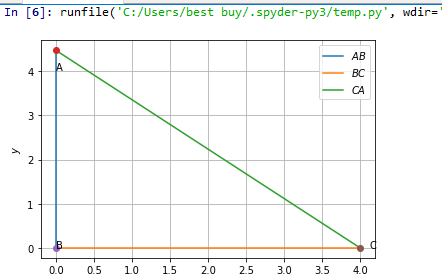
\includegraphics[width=10cm]{triangle.png}
	\caption{Fig generated using python}
\end{figure}
\newpage
\section{Construct an isosceles right angled $\Delta$ABC right
	angled at C such AC = 6.}
\subsection{Solution:-}
Given $\Delta$ABC isosceles right angled $\Delta$ at C such that AC=b=6, therefore , BC=a=6\\
Thus using Pyth. Theorem:\\
$AB^2$=$BC^2$+$AC^2$\\
$c^2$=$a^2$+$b^2$\\
c=8.48\\
	\paragraph{$\Delta$ABC is required triangle.}
\begin{tikzpicture}[scale=1]
	
	%Triangle sides
	\def\b{6}
	\def\c{8.48}
	\def\a{6}
	%Marking coordiantes
	\coordinate [label=below:$B$] (B) at (\a,0);
	\coordinate [label=left:$A$] (A) at (0,\b);
	\coordinate [label=left:$C$] (C) at (0,0);
	
	%Drawing triangle ABC
	\draw (B) -- node[above right] {$\textrm{c=8.48}$} (A) -- node[left] {$\textrm{b=6}$} (C) -- node[below,,xshift=2mm] {$\textrm{a=6}$} (B);
\end{tikzpicture}
\subsection{Output of Python code:-}
\begin{figure}[htp]
	\centering
	\includegraphics[width=10cm]{triangle-5.png}
	\caption{Fig generated using python}
\end{figure}
\end{document}